\section{Metodología}

\begin{frame}
	\frametitle{Metodología}
	La metodología realizada fue la siguiente:
	
	\begin{enumerate}
		\item Preprocesamiento de imágenes satelitales 
		\item Aplicación del Índice EVI 
		\item Método Random Forest
		\item Validación de resultados
	\end{enumerate}
\end{frame}

%---------------------------------------------------------
{
	\setbeamertemplate{background canvas}
	{
		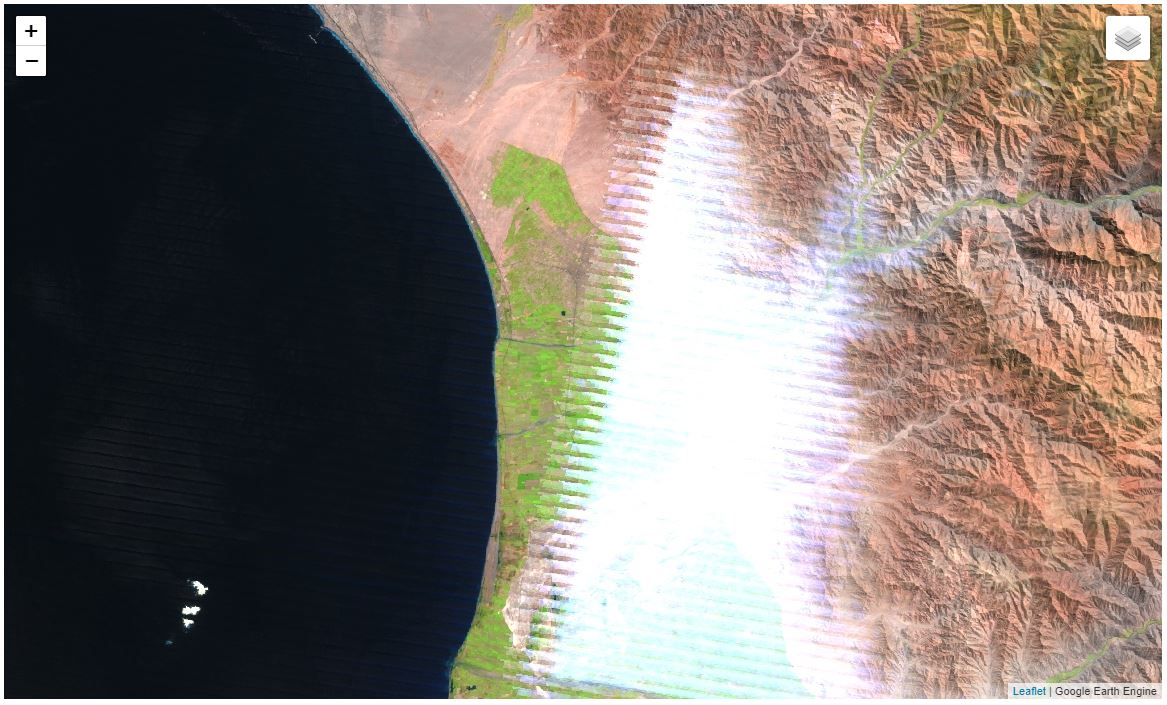
\includegraphics[width=\paperwidth,height=\paperheight]{imgs/pre_process_1.JPG}
	}
	\begin{frame}{Landsat 7 ETM sin tratar}
	\end{frame}
}
%---------------------------------------------------------
{
	\setbeamertemplate{background canvas}
	{
		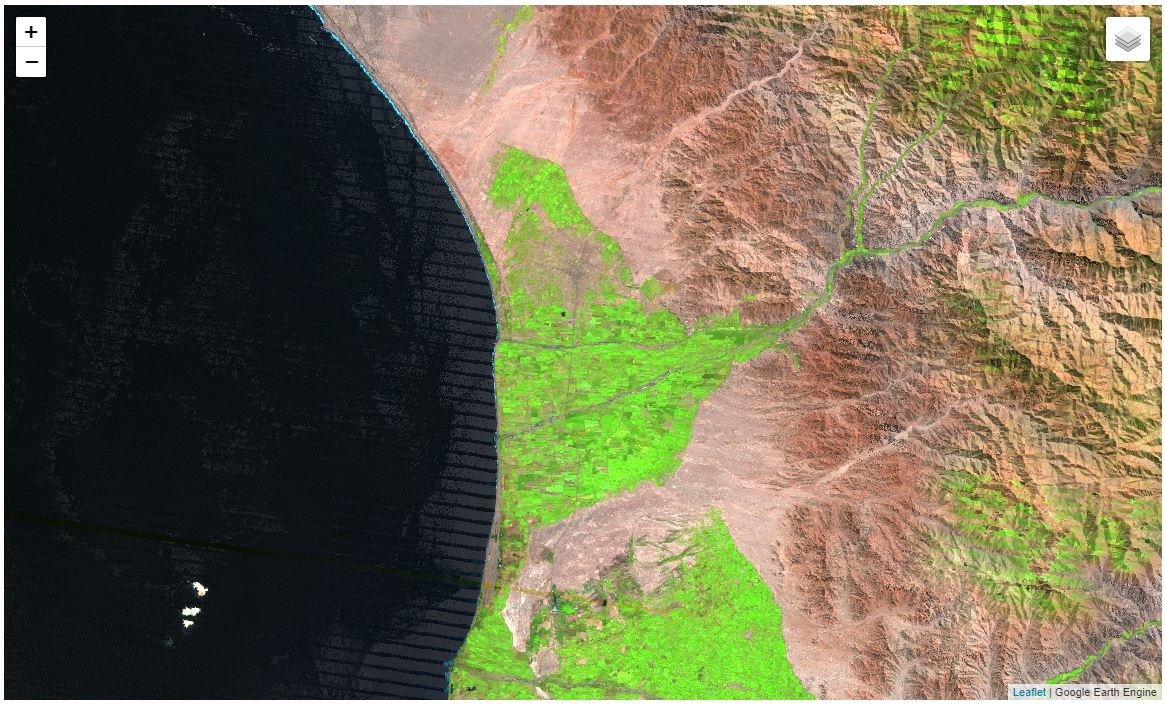
\includegraphics[width=\paperwidth,height=\paperheight]{imgs/pre_process_2.JPG}
	}
	\begin{frame}{Landsat 7 ETM tratada}
	\end{frame}
}
%--------------------------------------------------------
{
	\setbeamertemplate{background canvas}
	{
		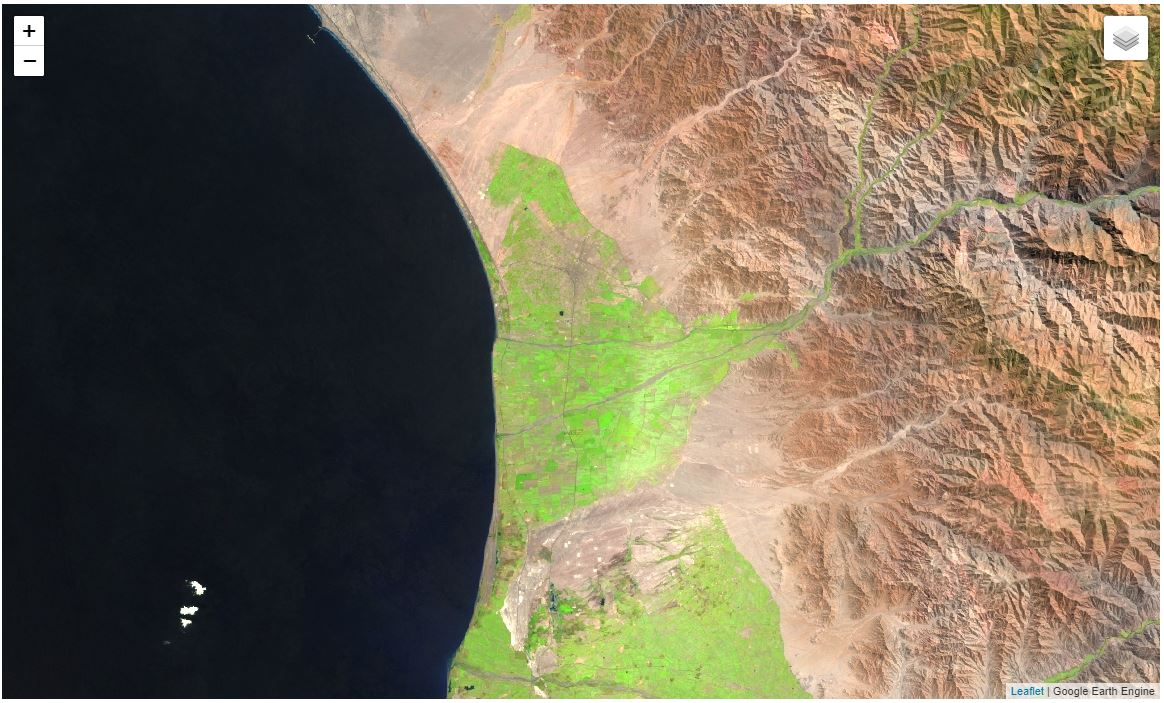
\includegraphics[width=\paperwidth,height=\paperheight]{imgs/pre_process_3.JPG}
	}
	\begin{frame}{Evaluando otros productos disponibles - Landsat 8}
	\end{frame}
}
%--------------------------------------------------------
\begin{frame}{Indice de Vegetación Mejorado - EVI}
	\begin{figure}
		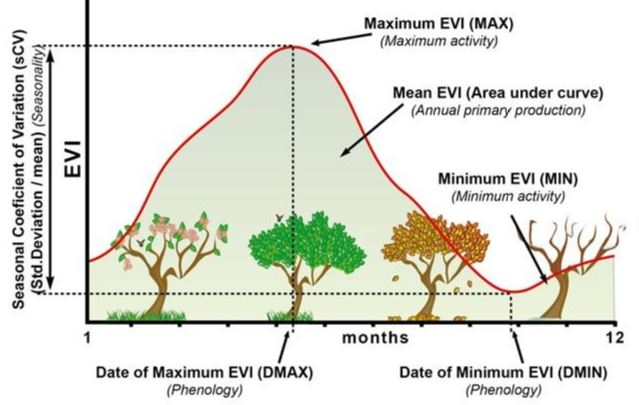
\includegraphics[scale=0.55]{imgs/EVI.JPG}
		\caption{EVI}
	\end{figure}
\end{frame}
%--------------------------------------------------------

\begin{frame}{Aplicación del EVI}
	\begin{figure}
		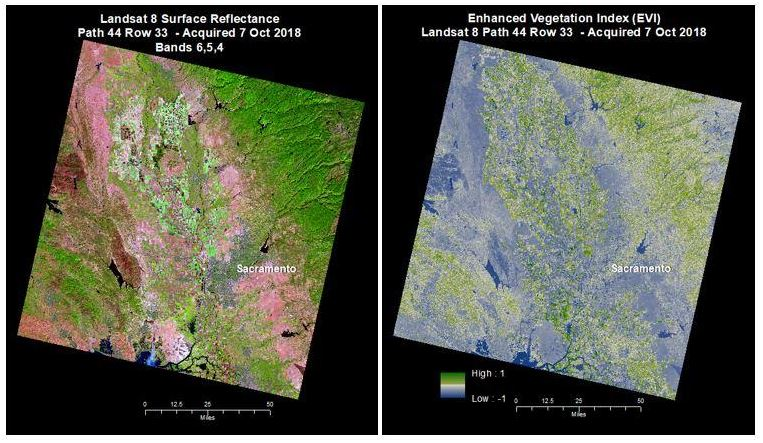
\includegraphics[scale=0.5]{imgs/EVI_result.JPG}
		\caption{Fuente: USGS}
	\end{figure}
\end{frame}
%--------------------------------------------------------

\begin{frame}{Método Random Forest}
	\begin{figure}
		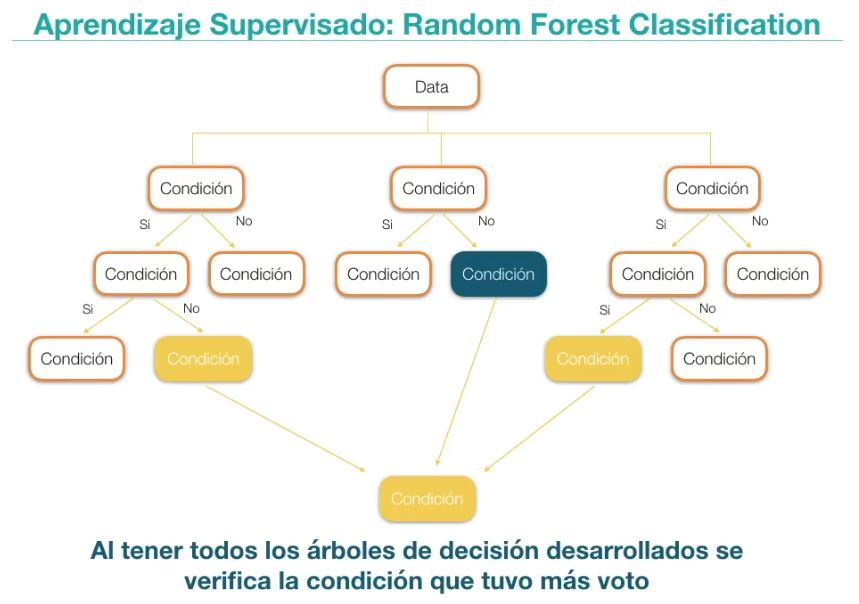
\includegraphics[scale=0.4]{imgs/random_forest.JPG}\\
		\caption{Curso de Introducción a Machine Learning - Ligdi Gonzalez - Youtube}
	\end{figure}
\end{frame}

%--------------------------------------------------------

\begin{frame}{Método Random Forest}
	\begin{figure}
		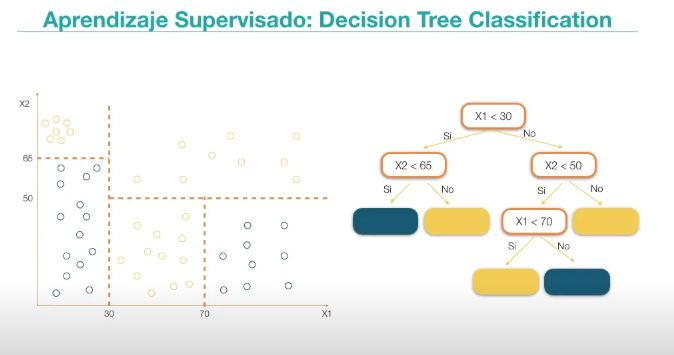
\includegraphics[scale=0.6]{imgs/random_forest_1.JPG}\\
		\caption{Curso de Introducción a Machine Learning - Ligdi Gonzalez - Youtube}
	\end{figure}
\end{frame}